\begin{figure}
\centering
\begin{tikzpicture}
  \node {
    \begin{tikzpicture}
      \node[inner sep=0pt] (circuit) at (0,0) {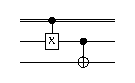
\includegraphics[scale=2]{Figures/circuits/classicalControl}};
      \node[right=0mm of circuit.north west, font=\itshape] (text) {a)};
    \end{tikzpicture}
    \hspace{8mm}
    \begin{tikzpicture}
      \node[inner sep=0pt] (circuit) at (0,0) {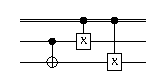
\includegraphics[scale=2]{Figures/circuits/classicalControl2}};
      \node[right=0mm of circuit.north west, font=\itshape] (text) {b)};
    \end{tikzpicture}
  };
\end{tikzpicture}
\caption{Pushing a classically controlled gate through a CNOT. The same rule as in Figure~\ref{fig:pullRules} is applied, while making sure any new gate is also controlled. Here, only the case for \(X\) gate is shown, but this works for any of the transformations in Figure~\ref{fig:pullRules}.}
\label{fig:classicalControl}
\end{figure}